% leastUPO.tex
%
% Predrag created file              Apr 12 2007
% $Author$ $Date$


\subsection*{Least unstable \rpo s ???}

\ES{
The names of the \rpo\ figure files follow the convention
 {\tt rpoL-T-d.eps}s, with suffixes {\tt cm}
and {\tt u} indicating
 mean velocity frame  and $u$ representation respectively.
   }
%
Out of 30 \rpo s we
find,  only three are periodic.  The orbit
with $\period{p} = 95.25$ has a very small
$d = -6.5\,\times 10^{-7}$, but it is not periodic
(we
checked this by decreasing the integration step size and increasing the
number of modes).


%%%%%%%%%%%%%%%%%%%%%%%%%%%%%%%%%%%%%%%%%%%%%%%%%%%%%%%%%%%%%%%%
\begin{figure}[t] \label{f:rpo55}
\begin{center}
(a) 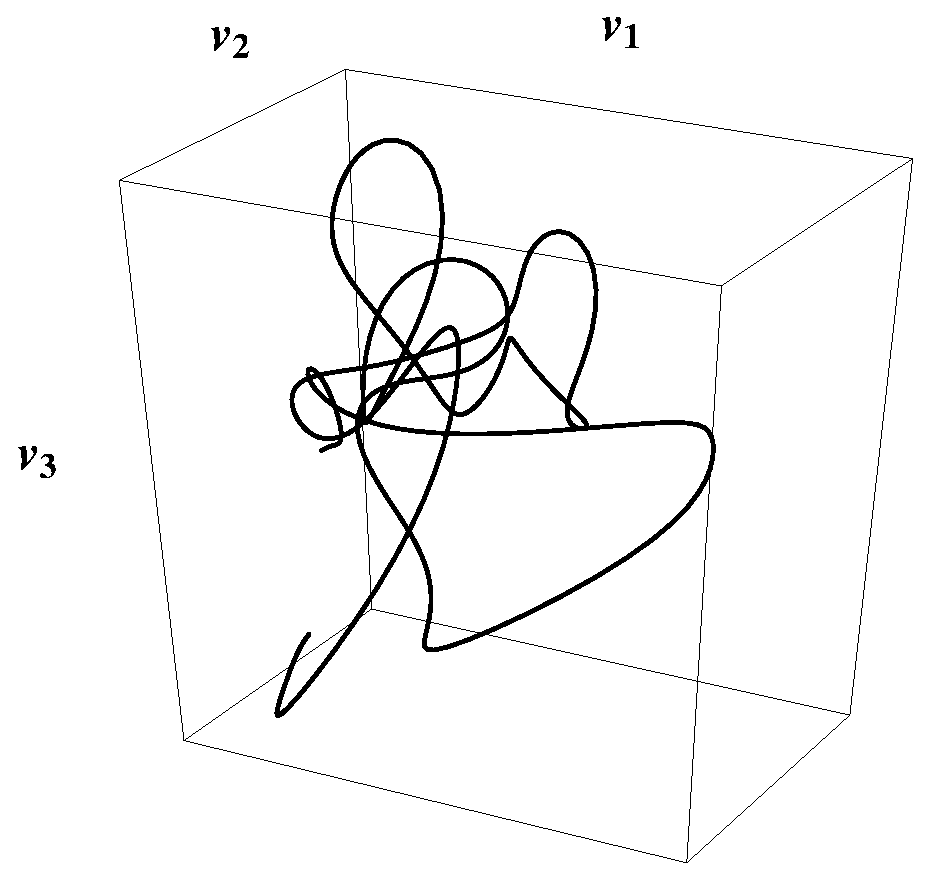
\includegraphics[width=0.35\textwidth]{figs/ks22rpo033.50_04.045E2.eps}
(b) 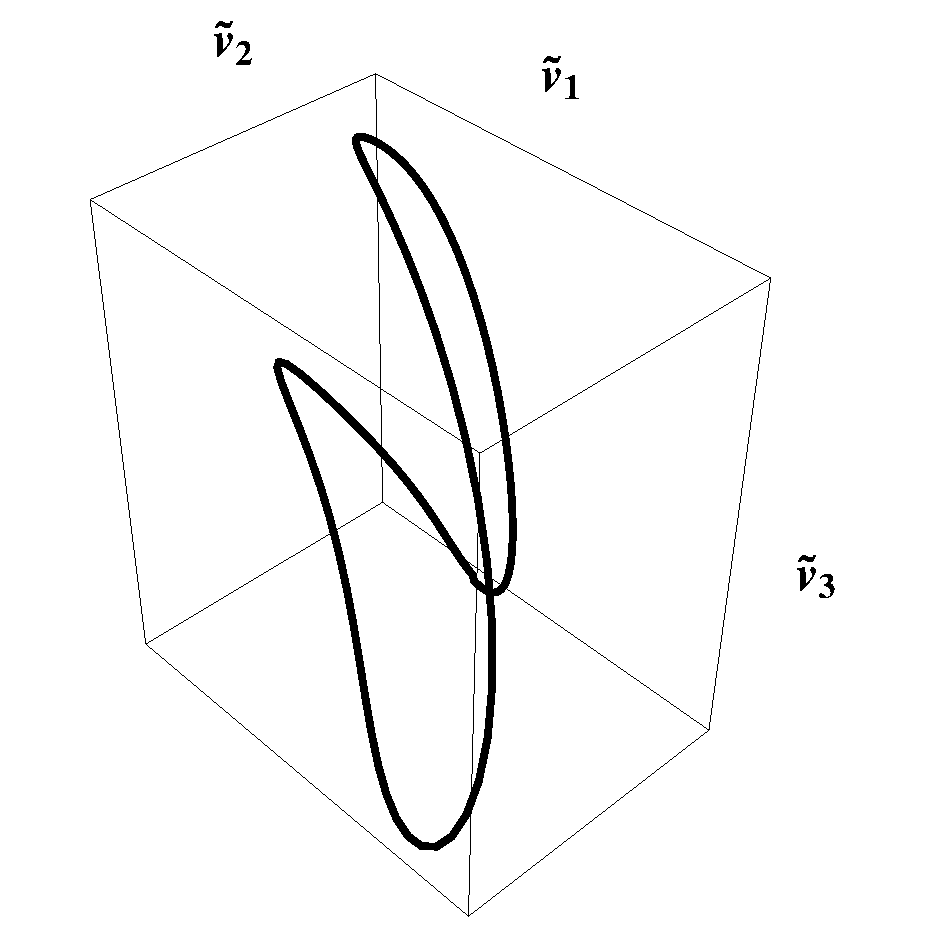
\includegraphics[width=0.35\textwidth]{figs/ks22rpo033.50_04.045E2CM.eps}
\\
\end{center}
\caption{
 The
which appears well embedded within the turbulent flow.
\rpo\ with $(\period{p},\shift_p) =(33.5,4.04)$
from \reffig{f:ks22rposShort}\,(\textit{c}) in:
 (a) \Statesp, traced for four periods $\period{p}$. The coordinate axes
$v_1$, $v_2$, and $v_3$ are those of \reffig{f:KS22E2man}.
 (b) Mean velocity frame.
        }
\end{figure}
%%%%%%%%%%%%%%%%%%%%%%%%%%%%%%%%%%%%%%%%%%%%%%%%%%%%%%%%%%%%%%%%%%



Sets of \rpo s are difficult to visualize simultaneously.

options:

Somewhat better visualization is in the
{\em mean velocity frame}, {\ie},
a reference frame that rotates with with velocity
$v_p=\shift_p/\period{p}$.
In the mean velocity frame a \rpo\ becomes
a \po, see  for example \refeq{f:rpo55}.
    \PC{
    I ordered a new laptop so I can open this mega.pdf,
but until that time, I can only look separately
at the individual figures in
\reffig{f:rpo55}.
    They seem to illustrate the idea nicely.
   Re. \reffig{f:rpo55}: Why not take
 the \rpo\ $(\period{p},\shift_p) =(32.8,10.96)$ from
 \reffig{f:ks22rposShort}\,(\textit{c}).
 \\
 BTW, are you sure that this is not
 $(\period{p},\shift_p) =(32.8,11)$? It is suspiciously close
 to $2\period{p}$ \po.
   }
Mean velocity frame visualization helps quite a bit.
Put a black (green, respectively) dot
twice thickness of the line every time unit; it will enable you to see
where the motion is slow and where it is fast.
% (a trick we used to understand plane Couette trajectories).
Mark the initial point on both
mean velocity \rpo\ and on \eqv\  in mean velocity
 frame with a fat triangle
indicating the direction, so we can see how they both move. Probably at the
opposite ends of the two curves - mean velocity frame is the mean motion.

%   rpo/figs/detail1rpo22-55-4.eps
%   rpo/figs/detail2rpo22-55-4.eps
%   rpo/figs/detail3rpo22-55-4.eps
%   break rpo22-55-4 into 3 parts.
%   The script for the fonts somehow crops these images

Each {\rpo} has its own mean velocity frame - and within it, {\eqv}
move on circles (or worse - because in higher Fourier modes they do more
complicated things), and it is important to know where the {\eqv} is at
a given instant.

As the shift $d$ is defined mod~$L$, better to
state for each {\rpo} its mean velocity $c_p = \shift_p/\period{p}$,
where $\shift_p$ is measured on the line (not on the circle). $c_p$ is
preferable to angle $2\pi \shift_p/L$ as it does not vary in $L \to$~large
limit (just like $\sqrt{2}$ wavelength estimate is independent of
system size).

Another convenient way to plot \eqva\ and \reqva\ on a periodic
domain $L$ is to plot
$u_x$ {\em vs.} $u$ as a curve parametrized by
$x\in [0,L]$.
In this representation both \eqva\ and \reqva\ curves are
stationary, but the \reqva\ points move as functions of time.

\Po s and \rpo s can be plotted this way, as well
$u_x(x,t)$ vs. $u(x,t)$. \Po s and \rpo s  in this representation
are time-dependent `tubes,' and distances between their instantaneous
profiles possible could serve to define `nearby' orbits for
flows with continuous symmetries.
